%%%%%%%%%%%%%%%%%%%%%%%%%%%%%%%%%%%%%%%%%%%%%%%%%%%%%%%%%%%%%%%%%%%%%
%                                                                   %
% NB: must be compiled with pdflatex -shell-escape poster_portrait  %
%                                                                   %
%%%%%%%%%%%%%%%%%%%%%%%%%%%%%%%%%%%%%%%%%%%%%%%%%%%%%%%%%%%%%%%%%%%%%

\documentclass[a0paper,portrait,fontscale=0.35]{baposter}

\usepackage{xeCJK}
%\usepackage{CJK} % CJK 中文支持                                  %
\usepackage{fontspec} % use to set font
\XeTeXlinebreaklocale "zh"  % Auto linebreak for chinese
\XeTeXlinebreakskip = 0pt plus 1pt % Auto linebreak for chinese
\setCJKfamilyfont{song}{SimSun}                             %宋体 song  
\newcommand{\song}{\CJKfamily{song}}                        % 宋体   (Windows自带simsun.ttf)  
\setCJKfamilyfont{xs}{NSimSun}                              %新宋体 xs  
\newcommand{\xs}{\CJKfamily{xs}}  
\setCJKfamilyfont{fs}{FangSong_GB2312}                      %仿宋2312 fs  
\newcommand{\fs}{\CJKfamily{fs}}                            %仿宋体 (Windows自带simfs.ttf)  
\setCJKfamilyfont{kai}{KaiTi_GB2312}                        %楷体2312  kai  
\newcommand{\kai}{\CJKfamily{kai}}                            
\setCJKfamilyfont{yh}{Microsoft YaHei}                    %微软雅黑 yh  
\newcommand{\yh}{\CJKfamily{yh}}  
\setCJKfamilyfont{hei}{SimHei}                                    %黑体  hei  
\newcommand{\hei}{\CJKfamily{hei}}                          % 黑体   (Windows自带simhei.ttf)  
\setCJKfamilyfont{msunicode}{Arial Unicode MS}            %Arial Unicode MS: msunicode  
\newcommand{\msunicode}{\CJKfamily{msunicode}}  
\setCJKfamilyfont{li}{LiSu}                                            %隶书  li  
\newcommand{\li}{\CJKfamily{li}}  
\setCJKfamilyfont{yy}{YouYuan}                             %幼圆  yy  
\newcommand{\yy}{\CJKfamily{yy}}  
\setCJKfamilyfont{xm}{MingLiU}                                        %细明体  xm  
\newcommand{\xm}{\CJKfamily{xm}}  
\setCJKfamilyfont{xxm}{PMingLiU}                             %新细明体  xxm  
\newcommand{\xxm}{\CJKfamily{xxm}}  
\setCJKfamilyfont{hwsong}{STSong}                            %华文宋体  hwsong  
\newcommand{\hwsong}{\CJKfamily{hwsong}}  
\setCJKfamilyfont{hwzs}{STZhongsong}                        %华文中宋  hwzs  
\newcommand{\hwzs}{\CJKfamily{hwzs}}  
\setCJKfamilyfont{hwfs}{STFangsong}                            %华文仿宋  hwfs  
\newcommand{\hwfs}{\CJKfamily{hwfs}}  
\setCJKfamilyfont{hwxh}{STXihei}                                %华文细黑  hwxh  
\newcommand{\hwxh}{\CJKfamily{hwxh}}  
\setCJKfamilyfont{hwl}{STLiti}                                        %华文隶书  hwl  
\newcommand{\hwl}{\CJKfamily{hwl}}  
\setCJKfamilyfont{hwxw}{STXinwei}                                %华文新魏  hwxw  
\newcommand{\hwxw}{\CJKfamily{hwxw}}  
\setCJKfamilyfont{hwk}{STKaiti}                                    %华文楷体  hwk  
\newcommand{\hwk}{\CJKfamily{hwk}}  
\setCJKfamilyfont{hwxk}{STXingkai}                            %华文行楷  hwxk  
\newcommand{\hwxk}{\CJKfamily{hwxk}}  
\setCJKfamilyfont{hwcy}{STCaiyun}                                 %华文彩云 hwcy  
\newcommand{\hwcy}{\CJKfamily{hwcy}}  
\setCJKfamilyfont{hwhp}{STHupo}                                 %华文琥珀   hwhp  
\newcommand{\hwhp}{\CJKfamily{hwhp}}  
\setCJKfamilyfont{fzsong}{Simsun (Founder Extended)}     %方正宋体超大字符集   fzsong  

\usepackage{amsfonts,amsmath,amssymb}
\usepackage{graphicx,subcaption}

\usepackage{relsize}
\usepackage{natbib}
\usepackage{pgfplots}
\pgfplotsset{compat=1.9}
\pgfmathdeclarefunction{gauss}{2}{%
  \pgfmathparse{1/(#2*sqrt(2*pi))*exp(-((x-#1)^2)/(2*#2^2))}%
}


\usepackage{microtype}

\usepackage{environ}
\makeatletter
\newsavebox{\measure@tikzpicture}
\NewEnviron{scaletikzpicturetowidth}[1]{%
  \def\tikz@width{#1}%
  \def\tikzscale{1}\begin{lrbox}{\measure@tikzpicture}%
    \BODY
  \end{lrbox}%
  \pgfmathparse{#1/\wd\measure@tikzpicture}%
  \edef\tikzscale{\pgfmathresult}%
  \BODY
}
\makeatother


%%% Define a caption font
\newcommand{\mycaption}[1]{
  {
    \smaller
    \emph{#1}
  }
}

%%% Color Definitions %%%%%%%%%%%%%%%%%%%%%%%%%%%%%%%%%%%%%%%%%%%%%%%%%%%%%%%%%
\definecolor{oxford_blue}{RGB}{14,31,71}
\definecolor{oxford_border}{RGB}{14,31,71}

\begin{document}
\typeout{Poster rendering started}

\begin{poster}
  {
    % Show grid to help with alignment
    grid=false,
    columns=4,
    % Column spacing
    colspacing=0.7em,
    % Color style
    % headerColorOne=cyan!20!white!90!black,
    % borderColor=cyan!30!white!90!black,
    headerColorOne=oxford_blue,
    borderColor=oxford_border,
    headerFontColor=white,
    % Format of textbox
    textborder=faded,
    % Format of text header
    headerborder=open,
    headershape=roundedright,
    headershade=plain,
    background=none,
    bgColorOne=cyan!10!white,
    headerheight=0.08\textheight
  }
  % Eye Catcher: Oxford logo and personal picture
  {
    \makebox[0.10\textwidth]{
%      \begin{tabular}{cc}
%        
\includegraphics[height=0.05\textheight]{./img/oxlogo}
      
\includegraphics[height=0.05\textheight,viewport=0 0 140 120,clip]{./img/BCC_logo-1.png}
 %        &
 %         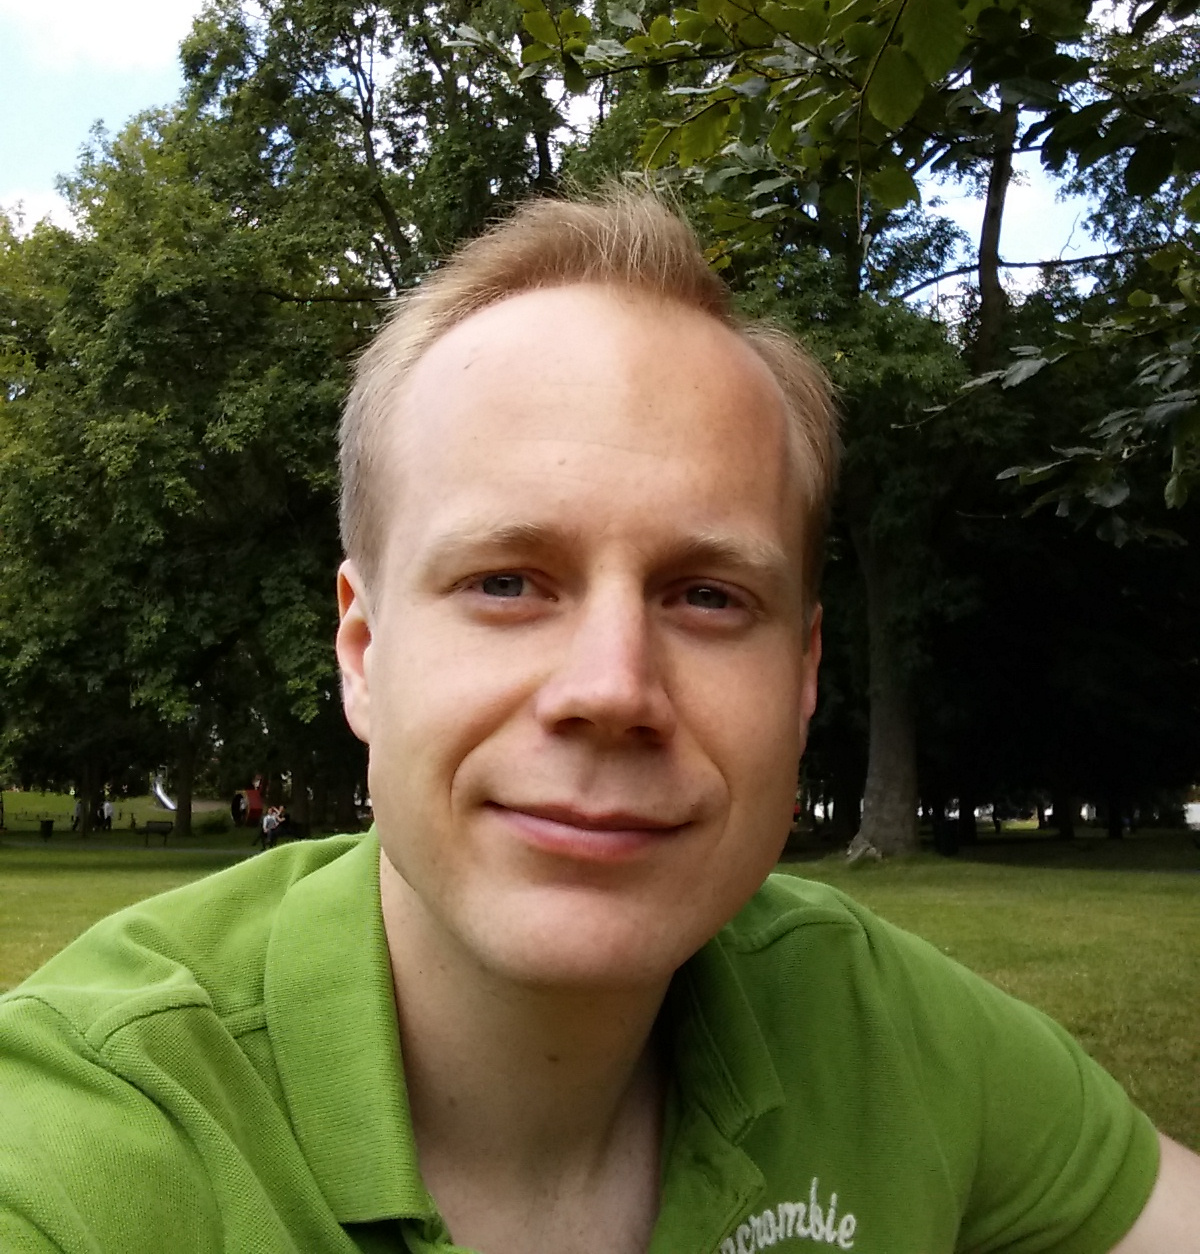
\includegraphics[height=0.05\textheight]{./img/profile}
%      \end{tabular}
%      \hfill
    }
  }
  %%% Title %%%%%%%%%%%%%%%%%%%%%%%%%%%%%%%%%%%%%%%%%%%%%%%%%%%%%%%%%%%%%%%%%%%%%
 % {\textsc{Pricing\,under\,uncertainty}}
  {\textsc{千原子量级模型高精度第一原理计算实现}}
  %%% Authors %%%%%%%%%%%%%%%%%%%%%%%%%%%%%%%%%%%%%%%%%%%%%%%%%%%%%%%%%%%%%%%%%%%
  {
    \vspace{0.5em}
%    Asbj{\o}rn Nilsen Riseth ---
 %   % \texttt{riseth@maths.ox.ac.uk}\\[0.1em]
%    \texttt{https://people.maths.ox.ac.uk/riseth}\\[0.1em]
%    { Mathematical Institute, University of Oxford}
    李计勇$^1$、李珅$^1$;~崔旭$^2$、姜骏$^2$\\[0.1em]
    1.~南京展智科技有限公司;~2.~北京市计算中心
  }
  %%% InFoMM Logo %%%%%%%%%%%%%%%%%%%%%%%%%%%%%%%%%%%%%%%%%%%%%%%%%%%%%%%%%%%%%%%
  {
    \makebox[0.23\textwidth]{
%      
\includegraphics[height=0.05\textheight]{./img/InFoMM}
      
\includegraphics[height=0.05\textheight,viewport=140 0 540 120,clip]{./img/BCC_logo-1.png}
    }
  }

  \headerbox{\hei 千原子量级模型计算的必要性和困难}{name=introduction,span = 2,column=0,row=0}{
	  {\hei 材料的属性由其基本组分、结构决定} \\[0.1em]
	  \includegraphics[height=0.064\textheight,width=0.340\textheight]{~/Documents/Latex_Beamer/Figures/MGE-2.png}
	  {\hei 材料模拟与计算在新材料研发中的作用日益凸显}:~%\textcolor{blue}
	  {功能材料}的属性精确调控:对材料组分与结构存在客观要求;%\textcolor{blue}
	  {结构材料}的微观缺陷和应力研究:对材料尺度也有客观要求;
	  \textrm{AI}支持的%textcolor{blue}
	  {跨尺度材料模拟}:对模型和数据同样有尺度要求。

	  \vspace{0.5em}
	  第一原理计算(主要是\textrm{DFT})为材料模拟提供``数据底座'':~包括微观电子结构在内的基本物性获得有效描述。\\[0.1em]
	  \includegraphics[height=0.192\textheight,width=0.340\textheight]{~/Documents/Latex_Beamer/Figures/Multi_Scale-5.jpg}

	  \vspace{0.5em}
	  {\hei \textrm{DFT}可精确模拟的材料尺度非常有限}\\[0.1em]
	  \includegraphics[height=0.110\textheight,width=0.170\textheight]{~/Documents/Latex_Beamer/Figures/Multi-Scale-6.png}
		\includegraphics[height=0.110\textheight,width=0.150\textheight]{~/Documents/Latex_Beamer/Figures/MLP_GNN.jpg}\\[0.1em]
	机器学习势函数,要考虑粒子间多体相互作用与长程相互作用

  }

  \headerbox{\hei \textrm{VASP}软件的主要瓶颈}
  {name=VASP-bottle-neck, column=0, below=introduction, above=bottom, span=2}
  {
	  \textrm{VASP}软件是维也纳大学\textrm{(Universit\"at Wien)}~\textrm{G. Kresse}等开发的第一原理模拟软件包,在物理方法、优化算法和并行计算实现等方面都有出色的性能:\\[-1.8em]%,是第一原理计算软件中``执牛耳''者
%	\begin{enumerate}
%\fontsize{7.2pt}{5.2pt}\selectfont
%		\item 采用\textrm{PAW~(Projector Augmented-Wave)}方法,平衡赝势方法和全电子计算优点,兼顾计算的精度和效率
%		\item 在实空间优化投影函数\textrm{(Projector)},将主要计算过程变换到实空间,节省内存开销%,保证了计算精度和效率
%		\item 引入多样的优化算法,提高矩阵对角化和电荷密度搜索的效率
%		\item 并行计算中有效均衡各节点处理\textrm{FFT}变换负载和通信,提升并行效率
%	\end{enumerate}
%	\vspace{-5.0em}
%    \begin{center}
	\includegraphics[height=0.150\textheight,width=0.170\textheight,viewport=0 0 240 200,clip]{~/Documents/Latex_Beamer/Figures/VASP-abinit_Li128-2.png}
	\includegraphics[height=0.135\textheight,width=0.170\textheight,viewport=0 0 240 180,clip]{~/Documents/Latex_Beamer/Figures/VASP-abinit_Li128-1.png}\\[0.1em]
%    \end{center}
	{\hei \textrm{VASP}计算的主要瓶颈:}内存、通信和\textrm{FFT}\\[-1.5em]
	\includegraphics[height=0.150\textheight,width=0.170\textheight,viewport=0 0 240 200,clip]{~/Documents/Latex_Beamer/Figures/VASP-mpi-Li128.png}
	\includegraphics[height=0.117\textheight,width=0.165\textheight,viewport=0 0 800 600,clip]{~/Documents/Latex_Beamer/Figures/dual_grid-2.png}\\
	{\hei \textrm{VASP}的\textrm{GPU}加速有限}\\[-0.1em]
	\includegraphics[height=0.095\textheight,width=0.34\textheight,viewport=0 0 850 260,clip]{~/Documents/Latex_Beamer/Figures/VASP-GPU-CPU.png}
  }

  \headerbox{\hei 针对\textrm{VASP}计算能力的提升策略}
  {name=furtherwork, column=2, row=0, span=2}
  {
	大规模\textrm{DFT}计算面临的效率问题,根源在于系统软件平台:\\{\fontsize{9.2pt}{7.2pt}\selectfont{
	传统系统软件平台难以充分发挥硬件性能,无法为\textrm{DFT}计算软件提供高效适配与支持。}}\\[0.2em]
	\textrm{VASP}软件将大模型的计算转化成矩阵基础操作:~%\\{\fontsize{7.2pt}{5.2pt}\selectfont{
	迭代对角化方案,依次(近似)求解矩阵本征值,因此单个本征值求解过程中,矩阵计算的相关性极高,参与计算的\textrm{CPU}核之间存在非常频繁的通信,产生极大的通信压力。\\[0.2em]%}}
%	\begin{itemize}
	{\fontsize{9.2pt}{7.2pt}\selectfont{
		%\item 
			如果多本征值并行求解,需要更多的系统资源来对多个本征值计算进行描述,模型越大,冗余开销越大;\\%,可能影响实用性,甚至超过了现有计算机集群的处理极限;\\
		%\item 
	如果把系统资源配置到单一本征值,会因算法失去局部性,各\textrm{CPU}核之间计算任务耦合过重。}}\\[0.2em]
%	\end{itemize}
	基于通用硬件搭建,通过优化系统软件层面对\textrm{DFT}计算的支持,释放\textrm{VASP}等软件的并行计算潜力,实现更大规模\textrm{DFT}模型的高效支持

	\vspace{0.5em}
	{\hei 主要技术难点}\\[0.3em]
	提升单个本征值求解的矩阵-向量乘处理极限,最大程度集成单个本征值计算的资源投入。
	\begin{itemize}
%			\fontsize{9.2pt}{7.2pt}\selectfont
			\item 高通量的分布式矩阵运算,会导致频繁的系统通信,在系统软件的临界区会产生严重冲突:~
				{\fontsize{9.2pt}{7.2pt}\selectfont{例如,多个计算节点同时请求访问共享资源、传输关键数据时,频繁的竞争与等待使得数据传输延迟大幅增加。}}
%构造一种新型通讯机制,兼容\textrm{DFT}计算的高通量矩阵需求与软件环境特征
		\item \textrm{VASP}软件基于\textrm{Intel}等基础库函数支持的并行计算库,在高并行度条件时,暴露出各种不适应:~
			{\fontsize{9.2pt}{7.2pt}\selectfont{例如,某些矩阵运算算法在多核心并行计算时,数据划分与同步机制不合理,导致核心间负载不均衡,大量核心处于空闲等待状态;部分通信算法在高并发数据传输时,因协议设计缺陷引发数据拥塞。}}
%			建立科学的算法评估体系,对这类不适用于高并行度的算法进行精准识别,并结合\textrm{DFT}计算特点,设计出适合高并行度的等效实现方案,从算法层面提升\textrm{VASP}软件在大规模并行计算中的性能表现
		\item \textrm{DFT}计算的核心数据结构的空间复杂度偏高:~
			{\fontsize{9.2pt}{7.2pt}\selectfont{\textrm{VASP}的部分核心数据结构的空间复杂度与$n^2$或$n^3$相关,当模型规模逐步扩大达到一定程度时,对于内存储器的开销过大,即使整个集群的\textrm{CPU}核只用于处理一个本征态所需的矩阵运算,仍会面临所需内存不足的问题。}}
	\end{itemize}
%	\vspace{0.5em}
	{\hei 总体技术路线}\\[0.3em]
	自研的虚拟机技术,将硬件进行重新封装,通过一系列自研数据结构、算法与特定编程方法,改变硬件呈现的特性,面向高通量数据处理软件提供更高效的运行环境。
	\begin{itemize}
		\item 高通量并发计算系统:\\
			单一本征值计算过程矩阵运算的\textrm{CPU}核间高效配合问题
			\begin{enumerate}
\fontsize{9.2pt}{7.2pt}\selectfont
				\item 重新划分软件分层,严格控制临界区范围
				\item 与高通量通信硬件的深度适配
			\end{enumerate}
		\item 并行计算库:~与高通量通信硬件的深度适配
			\begin{itemize}
\fontsize{9.2pt}{7.2pt}\selectfont
				\item 数据处理分层化:~将部分计算任务的处理过程进行分层,在负载均担与实时性需求之间进行再平衡
				\item 计算去中心化:~去掉各种形式的``主结点'',部分算法进行``去中心化''重写
			\end{itemize}
		\item 内存溢出子系统:~%在计算机集群系统中,
			集成内存储器的规模超过一定范围后,成本会明显增加\\
			{\fontsize{9.2pt}{7.2pt}\selectfont{
				针对\textrm{DFT}运算的核心数据结构访问局部性与连续性,设计了内外存储器联动的算法:~%该算法
				\\精准捕捉数据访问的规律,保证算法执行效率下降不超过\textrm{20\%}的前提下,可处理规模为内存储器\textrm{200\%$\sim$1000\%}以上的数据结构,有效突破内存容量对大规模计算的制约}}
	\end{itemize}
  }

  \headerbox{\hei 算例展示}
  {name=uncertainty, column=2, span=2, below=furtherwork}
  {
	 {\hei 三类模型}\\[-2.2em]
\includegraphics[height=0.061\textheight,width=0.11\textheight,viewport=0 100 656 429,clip]{~/Documents/Latex_Beamer/Figures/VASP_huge_SJTU-CdHgTe_POSCAR.png}
\includegraphics[height=0.063\textheight,width=0.11\textheight,viewport=0 150 726 519,clip]{~/Documents/Latex_Beamer/Figures/VASP_huge_USTB-CFeTi_POSCAR.png}
\includegraphics[height=0.043\textheight,width=0.11\textheight,viewport=0 320 680 543,clip]{~/Documents/Latex_Beamer/Figures/VASP_huge_Ningde-PbONICH_POSCAR.png}\\[0.3em]
{控制参数和并行规模}\\[-1.8em]
\begin{center}
\includegraphics[height=0.070\textheight,width=0.040\textheight,viewport=0 15 177 366,clip]{~/Documents/Latex_Beamer/Figures/VASP_huge_INCAR.png}\hspace{3.0em}
\includegraphics[height=0.070\textheight,width=0.160\textheight,viewport=0 350 735 645,clip]{~/Documents/Latex_Beamer/Figures/VASP_huge_OUTCAR.png}
\end{center}
\vspace{-1.0em}
{数据展示:~\textrm{CdHgTe}}\\[-1.8em]
\begin{center}
\includegraphics[height=0.061\textheight,width=0.15\textheight,viewport=0 50 1000 650,clip]{~/Documents/Latex_Beamer/Figures/VASP_huge_SJTU-CdHgTe_OSZICAR.png}
\includegraphics[height=0.061\textheight,width=0.13\textheight,viewport=0 0 1068 1059,clip]{~/Documents/Latex_Beamer/Figures/VASP_huge_SJTU-CdHgTe_OUTCAR-3.png}\\
\end{center}
\vspace{-1.0em}
{数据展示:~\textrm{CFeTi}}\\[-1.8em]
\begin{center}
\includegraphics[height=0.061\textheight,width=0.15\textheight,viewport=0 150 1000 500,clip]{~/Documents/Latex_Beamer/Figures/VASP_huge_USTB-CFeTi_OSZICAR.png}
\includegraphics[height=0.061\textheight,width=0.13\textheight,viewport=0 0 1046 1217,clip]{~/Documents/Latex_Beamer/Figures/VASP_huge_USTB-CFeTi_OUTCAR-1.png}\\
\end{center}
\vspace{-1.0em}
{数据展示:~\textrm{PbONICH}}\\[-2.4em]
\begin{center}
\includegraphics[height=0.120\textheight,width=0.11\textheight,viewport=0 0 1000 1152,clip]{~/Documents/Latex_Beamer/Figures/VASP_huge_Ningde-PbONICH_OUTCAR.png}
\end{center}
  }


%  \headerbox{Acknowledgements}
%  {name=acknowledgements, column=3, below=uncertainty, above=bottom, span=1}
%  {
%    \vspace{1em}
%    \begin{center}
%      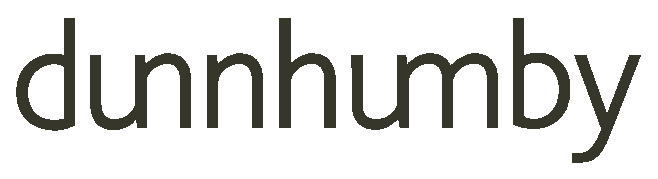
\includegraphics[width=0.65\textwidth]{./img/company_logo.eps}\\[1.5em]
%      
\includegraphics[width=0.65\textwidth]{./img/epsrc_logo.eps}
%    \end{center}
%  }
%
%  \headerbox{References}
%  {name=references, column=2, below=uncertainty, above=bottom, span=1}
%  {
%    \smaller                                  % Make the whole text smaller
%    \bibliographystyle{abbrv}                 % Use plain style
%    \renewcommand{\section}[2]{\vspace{0.05em}} % Omit "References" title
%    \bibliography{references}
%  }

\end{poster}
\end{document}

%%% Local Variables:
%%% mode: latex
%%% TeX-master: t
%%% End:
